\section{Methods}

\subsection{Overview}
Most approaches to the Super Resolution problem (especially GANs) are run on
datasets such as MNIST and CelebA. While those datasets excel at showing the
differences in image quality, they are not very representative of the real
world. In this problem, we attempt to tackle the super resolution of complex
images by breaking down the process into multiple steps:

\begin{enumerate}
	\item Segment the images into known classes
	\item Run the segmented images through a Super Resolution Conditional Generative Adversarial Network
	\item Run the non-segmented parts of the image into a standard bicubic interpolation function
	\item Merge the images together through image stitching

\end{enumerate}

\begin{figure}
	\centering
	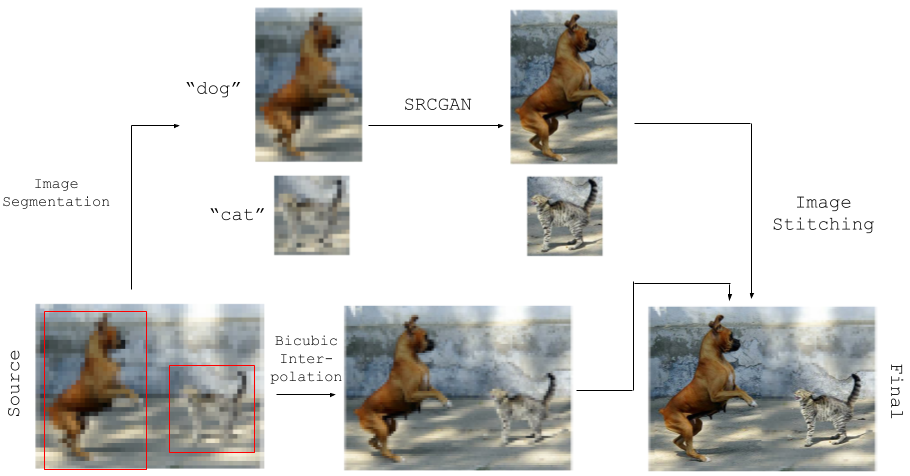
\includegraphics{images/intuition.png}
	\caption{An example of how our technique would work end-to-end. The source
	image (bottom right) would first be put through an Image Segmentation
	algorithm to determine the different subjects in the image. Once the subjects
	and their classes have been determined, they are then run through the SRCGAN.
	In the meanwhile, the whole image is run through a bicubic interpolation. Once
	the higher quality images have been formed, they are merged together through
	the image stitching algorithm. Once the images have been stitched together,
	the final image will be formed.}
	\label{fig:intuition}
\end{figure}

This process is illustrated by Figure \ref{fig:intuition}. By breaking the process up into smaller, more manageable chunks, one is able to take advantages of the different top-performing models. The following sections will go into greater detail on the reasons behind choosing the various methods and how they were implemented.

\subsection{Dataset Selection}

We opted to select datasets with one to three subjects in it in order present
where our proposed solution would shine. The datasets we selected for training
were created by splitting open source HD footage frame by frame. This allowed us
to create large easy to label datasets with ease.

\subsection{Segmentation}
\subsubsection{Fully Convolutional Network}

Fully Convolutional Network (FCN) is one of the states of the art techniques for
semantic segmentation. Semantic segmentation \cite{Liu2018} refers to the process of
associating each pixel in an image with a class label such as animals, roads,
buildings, etc. FCNs build up on CNN. CNNs are very good for image
classification data but they do not retain any spacial information with
convolutions. All the features are detected but their locations in the image are
not maintained. FCNs improve on this by just having convolutional layers. A
typical FCN network consists of an encoder block, 1x1 convolutional layer,
decoder block. The encoder block is pretty much the same as a CNN without the
fully connected layers. It downsamples the image with each convolution and
increases the feature maps. 1x1 convolutions are used to change the filter
dimensionality (either increase it or decrease it) before sending it to the
decoder block. The decoder block consists of transposed convolutional layers
often called deconvolutional layers. This part of the network deals with
upsampling the image to its original size. The output at the end is a image
associating each pixel with a class.

\begin{figure}
	\centering
	
	\begin{subfigure}[h]{0.4\textwidth}
		\centering
		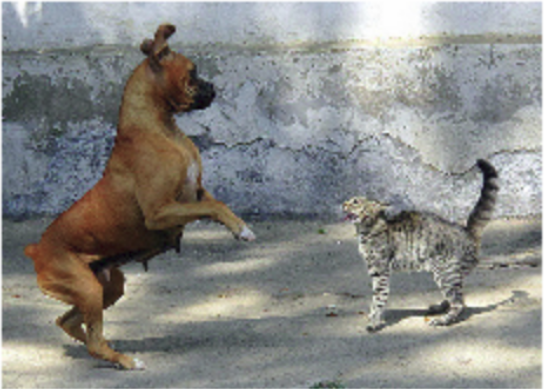
\includegraphics[width=\textwidth]{images/fcn-before.png}
		\caption{The source image fed into Google's DeepLab FCN.}
		\label{fig:fcn-before}
	\end{subfigure}

	\begin{subfigure}[h]{0.4\textwidth}
		\centering
		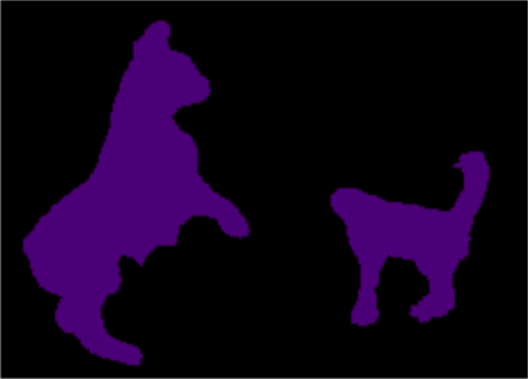
\includegraphics[width=\textwidth]{images/fcn-segmap.png}
		\caption{FCN's classification results. All of the subjects of interest are
		in purple, while the background is black.}
		\label{fig:fcn-segmap}
	\end{subfigure}

	\begin{subfigure}[h]{0.4\textwidth}
		\centering
		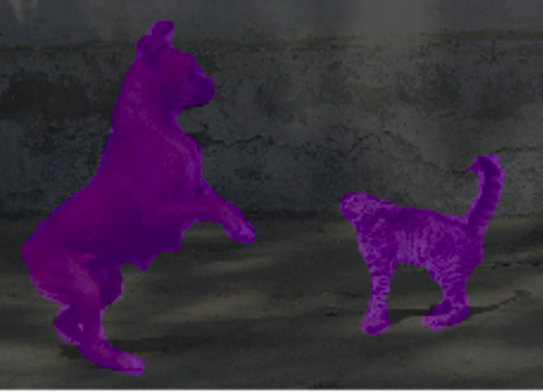
\includegraphics[width=\textwidth]{images/fcn-overlay.png}
		\caption{The FCN results overlayed on the original image.}
		\label{fig:fcn-overlay}
	\end{subfigure}

	\caption{Google's DeepLab Fully Convolutional Network.}
	\label{fig:fcn}
\end{figure}

We decided to use google’s pre-trained DeepLab FCN \cite{Chen2017}. It is able to perform
semantic segmentation on 21 predefined classes. The dataset images are fed into
this network to get a semantic segmentation output for the backgrounds and
object of interest. These objects of interest are then cropped out as individual
images to be fed into the super-resolution algorithm. The intact background is
passed forwards as well to the further methods.


\subsection{Super Resolution}
\subsubsection{General Adversarial Networks}
General Adversarial Networks (GANs) were first introduced by Goodfellow et al.
in 2014 \cite{Goodfellow2014}. GANs were a new framework that trained generative
models using an adversarial process. Under this framework, there are two models:
a generative model $G$, which trains off of the data distribution, and a
discriminative model $D$, which determines whether a sample is real or has been
generated. Both of the models are trained simultaneously, resulting in a
two-player game of sorts. In this game, $G$ generates a sample and $D$ tries to
guess whether or not the sample is real or not. In order to beat $D$, $G$ has to
create samples that are closer to the data set. Conversely, in order to beat $G$,
$D$ has to become more selective on what is a truth or not. This back and forth
process can intuitively be expressed as a generic 2-player minmax game:

\begin{IEEEeqnarray}{rCl}
	\min_{G}\max_{D}(D, G) = \nonumber\\
	E_{x p_{data}}[\log(D(x))] + E_{z p_{z}(z)}[\log(1 - D(G(z)))]
\end{IEEEeqnarray}

\subsubsection{Conditional GANs}
Mirza and Osindero improved upon Goodfellow et al.’s vanilla GAN by simply
adding auxiliary features to inputted data \cite{Mirza2014}. These “conditioning
features” are added as inputs to both the discriminator and generator functions
as well as labels to the data. These modifications can be seen in the following
objective function:

\begin{IEEEeqnarray}{rCl}
	\min_G\max_D(D,G) = E_{x p_{data}}[\log(D(x|\mathbf{y}))] \nonumber\\
	+ E_{z p_z(z)}[\log(1 - D(G(z|\mathbf{y})))]
\end{IEEEeqnarray}

In which the auxiliary feature vector is represented by $\mathbf{y}$. \\

Mirza and Osindero were able to successfully generated MNIST digits conditioned
on both the MNIST dataset and the respective class labels. \cite{Mirza2014} \\


\subsubsection{Super Resolution with CGANs}
GANs are currently some of the top methods for super resolution and CGANs have
been shown to work well in combining GANs and auxiliary information. Chen et al.
combined the two ideas by using CGANs for image super resolution \cite{Chen}. In
their report, Chen et al. introduce two methods of introducing new features into
their Super Resolution GAN (SRGAN)\cite{Chen}:

\begin{enumerate}
	\item (SRCGAN) - Add the class information as another input feature.
	\item (SRGAN + Class Loss) - Create an independant classifier whose purpose is
		to determine if the generated image is of the correct class and factor that
		into the objective function.
\end{enumerate}

In this project, an SRCGAN was chosen due to its demonstrated accuracy
improvements over a vanilla GAN \cite{Chen}. As per Chen et Al.’s findings, the
objective function for this model is as follows:

\begin{IEEEeqnarray}{rCl}
	\min_{\Theta_G}\max_{\Theta_D}(D, G) = \nonumber\\
	E_{I^{HR}\sim p_{train}}(I^{HR})[\log(D_{\Theta_D}(I^{HR}, \mathbf{c}))] \nonumber\\
	+ E_{I^{LR}\sim p_G(I^{LR})}[\log(1 - D_{\Theta_G}(G_{\Theta_G}(I^{LR},
		\mathbf{c})), \mathbf{c})]
\end{IEEEeqnarray}

In which $\mathbf{c}$ is the conditional information, $D$ and $G$ are the
updated discriminator and generator functions, and $I^{HR}$ and $I^{LR}$ are the
high-resolution and low-resolution images, respectively.

For the creation of the SRCGAN, Linder-Norén’s implementation of the SRGAN
\cite{Linder-Noren} from Ledig et Al  was used as a bootstrap due to its success in
photo-realistic super resolution \cite{Ledig}. The class information of the sample
subject was then added as another feature to the input vector and the objective
function was modified to account for the change in the feature space.

While Chen et Al. discuss that using class data as auxillary inputs in the
SRCGAN is trivial, they were only working on the MNIST and CelebA datasets
\cite{Chen}. In this case, it is trivial to see how class information (such as
“person”) would be a trivial feature to add, as all of the samples would share
the same information \cite{Chen}. However, this application hosts a variety of
different classes for subjects to be in, so including the class information
plays a non-trivial role. \\

\subsubsection{Bicubic Interpolation}
While GANs have made impressive advances in image super resolution, they are not
without fault. As Goodfellow discusses \cite{Goodfellow2017}, GANs tend to have
issues when dealing with:

\begin{itemize}
	\item Counting
	\item Perspective
	\item Global Structures
\end{itemize}

While these drawbacks may be a bit more trivial when working on more restrictive
datasets such as MNIST or CelebA, they become more of an ordeal when dealing
with complex, multi-subject images. For that reason, the SR model chosen for the
base images was Lukin et al.’s Bicubic Interpolation SR model from 2006
\cite{Lukin2006}. The Bicubic Interpolation SR model has seen impressive results in a scaling
factor of 2x and is now considered a baseline SR model. For this project,
OpenCV’s bicubic interpolation implementation was used \cite{Bradski2000}.

\subsection{Image Stitching}
One side-effect of the processes described in this paper is that the subjects of
the image and the background are separated. As a result, the images need to be
stitched back together into one final product image. Python’s OpenCV library and
PIL (Python Imaging Library) are utilized to accomplish this task. Provided the
(x,y) coordinate and (width, height) of the extracted subject image from the
original image, PIL inserts the new subject images back into the main image at
their original locations. The data for this operation is retrieved during the
image segmentation process.

However, a simple copy/paste procedure wouldn’t be enough to truly recreate an
image. Since the background image and the subject images have different
resolutions, the combined image has the possibility of looking somewhat awkward
on the edge of the background and subject image from the sudden change in
resolution. OpenCV has functionality that can be implemented to blur parts of an
image with a certain intensity, which is used here to blur along the shared
edges with different intensity such that the transition from the background
image to subject image looks more natural.
